\documentclass[12pt]{article}
\pagestyle{empty}

% Fonts and Packages
\usepackage{amsmath}
\usepackage{amssymb}
\usepackage{amsfonts}
\usepackage{fancyhdr}
\usepackage{setspace}
\usepackage{titlesec}
\usepackage{enumitem}
\usepackage{caption}
\usepackage{booktabs}
\usepackage{geometry}
\usepackage{hyperref}
\usepackage{float}
\usepackage{array}
\usepackage{graphicx}
\usepackage{xcolor}
\usepackage{listings}


% % Bengali language support
% \usepackage{polyglossia}
% \setmainlanguage{english}
% \setotherlanguage{bengali}
% \newfontfamily\bengalifont{Noto Serif Bengali}[Script=Bengali]

% Language and fonts
\usepackage{polyglossia}
\setmainlanguage{english}
\setotherlanguage{bengali}

\usepackage{fontspec}

% English font (Palatino-like options)
\setmainfont{TeX Gyre Pagella} % Best Palatino alternative (included with TeX Live/MiKTeX)
%\setmainfont{Palatino Linotype} % Windows default Palatino
%\setmainfont{Book Antiqua} % Another Palatino-inspired option
%\setmainfont{EB Garamond} % Classical serif, if you want a Garamond look
%\setmainfont{Charter} % Clean, wide serif, very readable

% Bengali font
\newfontfamily\bengalifont{Noto Serif Bengali}[Script=Bengali]

\geometry{margin=1in}

% Unnumbered sections
\titleformat{\section}
  {\normalfont\Large\bfseries}{\thesection}{1em}{}
\titlespacing*{\section}{0pt}{1.5ex plus 1ex minus .2ex}{1ex plus .2ex}

% Hyperlink setup
\hypersetup{
    colorlinks=true,
    linkcolor=blue,
    urlcolor=blue,
    citecolor=blue
}

% Listings setup for pseudocode - remove italics
\lstset{
    basicstyle=\ttfamily\small,
    breaklines=true,
    columns=fullflexible,
    frame=single,
    numbers=left,
    numberstyle=\tiny,
    tabsize=4,
    showstringspaces=false,
    language=Python,
    keywordstyle=\bfseries,
    commentstyle=\rmfamily,
    stringstyle=\rmfamily
}

\begin{document}

\section*{Introduction}
Next-word prediction is a key task in natural language processing (NLP), enabling applications such as text autocompletion, chatbots, and language modeling. This lab report details the development of a next-word prediction model for Bangla text, inspired by Ravjot Singh's blog, ``Mastering Next Word Prediction with Recurrent Neural Networks (RNNs) . Unlike the blog's simple Recurrent Neural Network (RNN), this model employs a Bidirectional Long Short-Term Memory (LSTM) architecture to capture contextual dependencies in both directions, addressing limitations like vanishing gradients. The model was trained on a Bangla dataset describing a fictional city, Kankapur, and achieved a training accuracy of 99.98\% with a loss of 0.0163 over 100 epochs. This report outlines the dataset, model architecture, training results, findings, and conclusions.

\section*{Dataset Details}
The dataset, stored in an Excel file (\texttt{somoresh.xlsx}), contains 2,478 Bangla words across narrative and dialogue segments about Kankapur, a fictional city known for its peaceful environment and tourism appeal. The dataset has four columns: \texttt{segment\_id}, \texttt{text}, \texttt{segment\_type} (narration or dialogue), and \texttt{metadata} (contextual descriptions). The \texttt{text} column was used for training, preprocessed to retain only Bangla characters , numbers, and punctuation (\texttt{.,?!}). The preprocessing yielded 2,473 sequences with a sequence length of 5 words and a vocabulary size of 1,168 unique words. Below Table Shows the first five dataset entries.

\begin{table}[H]
\centering
\caption{First Five Entries of the Bangla Dataset}
\label{tab:dataset_sample}
\begin{tabular}{|>{\raggedright\arraybackslash}p{1.5cm}|>{\raggedright\arraybackslash}p{6cm}|>{\raggedright\arraybackslash}p{2cm}|>{\raggedright\arraybackslash}p{3cm}|}
\hline
\textbf{Segment ID} & \textbf{Text} & \textbf{Segment Type} & \textbf{Metadata} \\
\hline
1 & {\bengalifont এরকম ঘটনা এই শহরে এর আগে ঘটেনি।} & Narration & Introduction, setting the premise \\
\hline
2 & {\bengalifont তার আগে শহরটার পরিচয় দেওয়া দরকার। আমাদের চেনাশোনা আর পাঁচটা শহরের সঙ্গে এই শহরটির পার্থক্য হল এখানে আইন-শৃঙ্খলা সবাই মানে, বয়স্কদের শ্রদ্ধা করে কনিষ্ঠরা, কারণ এই শহরটিকে ওঁরা নিজেদের রক্ত দিয়েই তৈরি করেছেন বলা যায়।} & Narration & Description of the city (Kankapur) \\
\hline
3 & {\bengalifont হিমালয়ের এই তল্লাটের আরও কিছু নামী-দামি শহর আছে যেখানে প্রতি বছর লক্ষ-লক্ষ মানুষ আসে টুরিস্ট হয়ে।} & Narration & Background: Tourism, reputation of water \\
\hline
4 & {\bengalifont সেই শহরে একদিন সকালে কাণ্ডটা ঘটে গেল।} & Narration & Incident: A young man runs to the police station \\
\hline
5 & {\bengalifont যুবকুটি হাঁপাতে হাঁপাতে বলল, অফিসার, আমার স্ত্রীকে বাঁচান।} & Dialogue & Young Man \\
\hline
\end{tabular}
\end{table}

\section*{Model Details}
The model is a Bidirectional LSTM neural network designed to predict the next word in a Bangla text sequence. It improves upon the simple RNN in   by using LSTM layers to handle long-range dependencies and bidirectional processing to capture context from both directions. The architecture consists of:

\begin{itemize}
    \item \textbf{Embedding Layer}: Maps 1,168 vocabulary words to 128-dimensional vectors, with an input length of 5 words.
    \item \textbf{Bidirectional LSTM}: 256 units, \texttt{return\_sequences=True}, to process sequences bidirectionally.
    \item \textbf{Dropout}: 30\% rate to prevent overfitting.
    \item \textbf{LSTM}: 256 units for further sequence processing.
    \item \textbf{Dropout}: 30\% rate.
    \item \textbf{Dense (ReLU)}: 256 units for non-linear feature extraction.
    \item \textbf{Dense (Softmax)}: 1,168 units to output probabilities over the vocabulary.
\end{itemize}

The model was compiled with \texttt{categorical\_crossentropy} loss, \texttt{adam} optimizer, and \texttt{accuracy} metric. It was trained on 2,473 sequences for 100 epochs with a batch size of 64, using \texttt{EarlyStopping} (patience=10, monitor \texttt{loss}) and \texttt{ReduceLROnPlateau} (patience=5, factor=0.5) callbacks. The pseudocode is shown below:

\begin{lstlisting}
Algorithm: BanglaNextWordPrediction

Input: 
  Excel file with Bangla text
  Sequence length = 5

Output: 
  Trained model, tokenizer, predictions

Steps:
1. Load Excel file using pandas.read_excel
2. Detect text column with Bangla characters (\u0980-\u09FF)
3. Clean text: keep Bangla characters, numbers, punctuation
4. Split text into words (2478 words)
5. Create sequences of length 5 (2473 sequences)
6. Tokenize sequences using Tokenizer (vocab_size = 1168)
7. Pad sequences (pre-padding) and one-hot encode outputs
8. Build model with layers:
   - Embedding(vocab_size, 128, input_length=5)
   - Bidirectional(LSTM(256, return_sequences=True))
   - Dropout(0.3)
   - LSTM(256)
   - Dropout(0.3)
   - Dense(256, activation='relu')
   - Dense(vocab_size, activation='softmax')
9. Compile model: 
   loss='categorical_crossentropy'
   optimizer='adam'
   metrics=['accuracy']
10. Train model: 
    epochs=100
    batch_size=64
    callbacks=[EarlyStopping, ReduceLROnPlateau]
11. Save model and tokenizer
12. Prediction process:
    - Input text, clean and tokenize
    - Pad sequence to length 5
    - Predict top 3 words using model.predict and np.argsort
    - Return predicted words
\end{lstlisting}

\section*{Findings}
The model was trained on 2,473 sequences, achieving a final accuracy of 99.98\% and a loss of 0.0163 after 100 epochs. The training took 57.56 seconds, with learning rate reductions at epochs 63 (to 0.0005) and 88 (to 0.00025) to optimize convergence. Key findings include:

\begin{itemize}
    \item \textbf{Training Performance}: The loss decreased from 7.0359 (epoch 1) to 0.0163 (epoch 100), and accuracy increased from 1.67\% to 99.98\%, indicating effective learning of dataset patterns. Figure \ref{fig:training_plots} shows the loss and accuracy curves.
    \item \textbf{Prediction Quality}: Interactive testing produced contextually relevant predictions in some cases (e.g., {\bengalifont ``তারপর''} for {\bengalifont ``জমিটা পেয়ে গেছি। টাউন কমিটি স্যাংশন করেছে। শিগগির কাজ শুরু করব।''}), but others were less accurate (e.g., {\bengalifont ``কাছে''} for {\bengalifont ``হঠাৎ সুর্মা বলে উঠল, জানো বাবা,''}), suggesting dataset bias or limited vocabulary diversity.
    \item \textbf{Limitations}: The high accuracy may indicate overfitting, as no validation split was used. The dataset's small size (2,478 words) limits generalization. Excluding the Bangla in preprocessing may have affected sentence boundary detection.
\end{itemize}

\begin{figure}[H]
    \centering
    \caption{Training Loss and Accuracy Over Epochs}
    \label{fig:training_plots}
    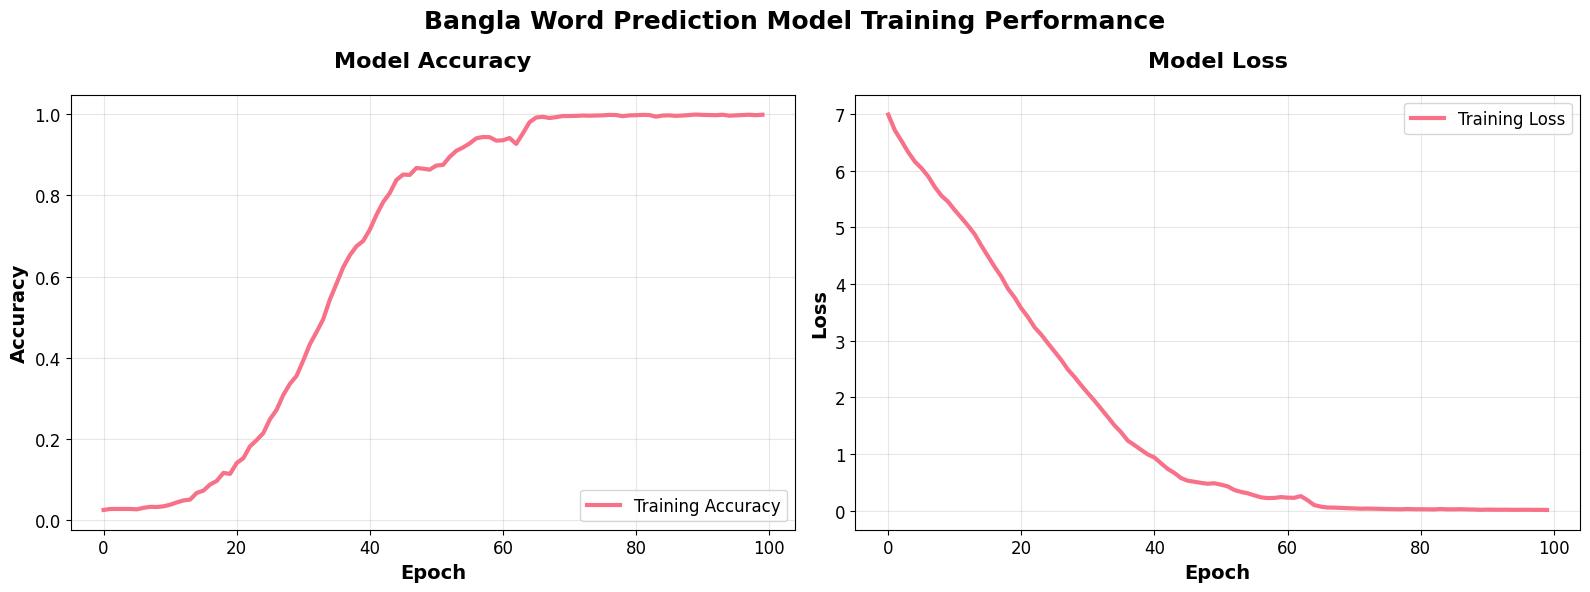
\includegraphics[width=1.0\textwidth]{curves.png}
\end{figure}

\section*{Conclusion}
The Bangla next-word prediction model, built with a Bidirectional LSTM, successfully learned patterns from a 2,478-word dataset, achieving 99.98 accuracy and 0.0163 loss. The model's predictions were moderately accurate but showed limitations due to the small dataset and potential overfitting. The use of Bidirectional LSTM and dropout improved upon the simple RNN , capturing contextual dependencies effectively. Future improvements should include a larger dataset, validation split, and pretrained Bangla embeddings to enhance prediction quality and generalization.


\end{document}